% !TEX root = main.tex
\section{Auswertung}
Im Folgenden werden die Auswertung der gewonnenen Daten sowie die Interpretation und Analyse der Ergebnisse dargelegt.
    \subsection{Beobachtung der Sonne}
    Dabei wird mit der Betrachtung der Sonne begonnen.
    Intention dessen war einerseits, die ,,antenna response function`` mittels Intensitätsmessungen zu ermitteln und
    daraus charakteristische Größen des Teleskops zu berechnen, und andererseits, als Grundlage hierfür die Annahme zu legitimieren,
    dass die Sonne innerhalb dieses Versuchs als Punktquelle aufgefasst wird.\\

    Um die Messungen der Intensitätsspektren der Sonne nicht durch charakteristische Radiostrahlung der
    21-\si{\centi \metre}-Linie zu beeinflussen,
    wurden diese bei einer Frequenz von $\SI{1410}{\mega \hertz}$ für jeweils $\SI{10}{\second}$ durchgeführt.
    Genauer wurde der Messprozess bereits in Abschnitt \ref{sec:Aufbau} beschrieben. 
    Beispielhaft zeigt Abbildung \ref{fig:Sonnenspektrum} eine solches Spektrum.
    Aus den gewonnenen Spektren wurde anschließend stets der Intensitätswert bei der Messefrequenz $\SI{1410}{\mega \hertz}$ ausgelesen, um eine Grundlage für die Vergleichbarkeit der Daten zu schaffen.  
    Diese Frequenz ist in Abbildung \ref{fig:Sonnenspektrum} hervorgehoben und zeigt, dass durch dieses Vorgehen mit guter Genauigkeit das Maximum des jeweiligen Spektrums erhalten wurde. 
    Dieses Verfahren wurde sowohl beim $5$$\times$$5$-Raster-Scan als auch bei den Kreuz-Scans angewendet.
    Die Intensitätswerte wurden in den entsprechenden Abbildungen \ref{fig:Sonnenabbild} bis \ref{fig:Sonnenkreuz_Alt} geplottet. 

    \begin{figure}[ht]
        \centering
        % GNUPLOT: LaTeX picture with Postscript
\begingroup
  % Encoding inside the plot.  In the header of your document, this encoding
  % should to defined, e.g., by using
  % \usepackage[cp1252,<other encodings>]{inputenc}
  \inputencoding{cp1252}%
  \makeatletter
  \providecommand\color[2][]{%
    \GenericError{(gnuplot) \space\space\space\@spaces}{%
      Package color not loaded in conjunction with
      terminal option `colourtext'%
    }{See the gnuplot documentation for explanation.%
    }{Either use 'blacktext' in gnuplot or load the package
      color.sty in LaTeX.}%
    \renewcommand\color[2][]{}%
  }%
  \providecommand\includegraphics[2][]{%
    \GenericError{(gnuplot) \space\space\space\@spaces}{%
      Package graphicx or graphics not loaded%
    }{See the gnuplot documentation for explanation.%
    }{The gnuplot epslatex terminal needs graphicx.sty or graphics.sty.}%
    \renewcommand\includegraphics[2][]{}%
  }%
  \providecommand\rotatebox[2]{#2}%
  \@ifundefined{ifGPcolor}{%
    \newif\ifGPcolor
    \GPcolorfalse
  }{}%
  \@ifundefined{ifGPblacktext}{%
    \newif\ifGPblacktext
    \GPblacktexttrue
  }{}%
  % define a \g@addto@macro without @ in the name:
  \let\gplgaddtomacro\g@addto@macro
  % define empty templates for all commands taking text:
  \gdef\gplbacktext{}%
  \gdef\gplfronttext{}%
  \makeatother
  \ifGPblacktext
    % no textcolor at all
    \def\colorrgb#1{}%
    \def\colorgray#1{}%
  \else
    % gray or color?
    \ifGPcolor
      \def\colorrgb#1{\color[rgb]{#1}}%
      \def\colorgray#1{\color[gray]{#1}}%
      \expandafter\def\csname LTw\endcsname{\color{white}}%
      \expandafter\def\csname LTb\endcsname{\color{black}}%
      \expandafter\def\csname LTa\endcsname{\color{black}}%
      \expandafter\def\csname LT0\endcsname{\color[rgb]{1,0,0}}%
      \expandafter\def\csname LT1\endcsname{\color[rgb]{0,1,0}}%
      \expandafter\def\csname LT2\endcsname{\color[rgb]{0,0,1}}%
      \expandafter\def\csname LT3\endcsname{\color[rgb]{1,0,1}}%
      \expandafter\def\csname LT4\endcsname{\color[rgb]{0,1,1}}%
      \expandafter\def\csname LT5\endcsname{\color[rgb]{1,1,0}}%
      \expandafter\def\csname LT6\endcsname{\color[rgb]{0,0,0}}%
      \expandafter\def\csname LT7\endcsname{\color[rgb]{1,0.3,0}}%
      \expandafter\def\csname LT8\endcsname{\color[rgb]{0.5,0.5,0.5}}%
    \else
      % gray
      \def\colorrgb#1{\color{black}}%
      \def\colorgray#1{\color[gray]{#1}}%
      \expandafter\def\csname LTw\endcsname{\color{white}}%
      \expandafter\def\csname LTb\endcsname{\color{black}}%
      \expandafter\def\csname LTa\endcsname{\color{black}}%
      \expandafter\def\csname LT0\endcsname{\color{black}}%
      \expandafter\def\csname LT1\endcsname{\color{black}}%
      \expandafter\def\csname LT2\endcsname{\color{black}}%
      \expandafter\def\csname LT3\endcsname{\color{black}}%
      \expandafter\def\csname LT4\endcsname{\color{black}}%
      \expandafter\def\csname LT5\endcsname{\color{black}}%
      \expandafter\def\csname LT6\endcsname{\color{black}}%
      \expandafter\def\csname LT7\endcsname{\color{black}}%
      \expandafter\def\csname LT8\endcsname{\color{black}}%
    \fi
  \fi
    \setlength{\unitlength}{0.0500bp}%
    \ifx\gptboxheight\undefined%
      \newlength{\gptboxheight}%
      \newlength{\gptboxwidth}%
      \newsavebox{\gptboxtext}%
    \fi%
    \setlength{\fboxrule}{0.5pt}%
    \setlength{\fboxsep}{1pt}%
\begin{picture}(7200.00,5040.00)%
    \gplgaddtomacro\gplbacktext{%
      \csname LTb\endcsname%%
      \put(814,704){\makebox(0,0)[r]{\strut{}$0$}}%
      \put(814,1253){\makebox(0,0)[r]{\strut{}$100$}}%
      \put(814,1801){\makebox(0,0)[r]{\strut{}$200$}}%
      \put(814,2350){\makebox(0,0)[r]{\strut{}$300$}}%
      \put(814,2899){\makebox(0,0)[r]{\strut{}$400$}}%
      \put(814,3447){\makebox(0,0)[r]{\strut{}$500$}}%
      \put(814,3996){\makebox(0,0)[r]{\strut{}$600$}}%
      \put(814,4545){\makebox(0,0)[r]{\strut{}$700$}}%
      \put(946,484){\makebox(0,0){\strut{}$1408.5$}}%
      \put(1922,484){\makebox(0,0){\strut{}$1409$}}%
      \put(2898,484){\makebox(0,0){\strut{}$1409.5$}}%
      \put(3875,484){\makebox(0,0){\strut{}$1410$}}%
      \put(4851,484){\makebox(0,0){\strut{}$1410.5$}}%
      \put(5827,484){\makebox(0,0){\strut{}$1411$}}%
      \put(6803,484){\makebox(0,0){\strut{}$1411.5$}}%
    }%
    \gplgaddtomacro\gplfronttext{%
      \csname LTb\endcsname%%
      \put(308,2761){\rotatebox{-270}{\makebox(0,0){\strut{}Temperatur in K}}}%
      \put(3874,154){\makebox(0,0){\strut{}Frequenz in mHz}}%
      \csname LTb\endcsname%%
      \put(5816,4646){\makebox(0,0)[r]{\strut{}Messwerte}}%
    }%
    \gplbacktext
    \put(0,0){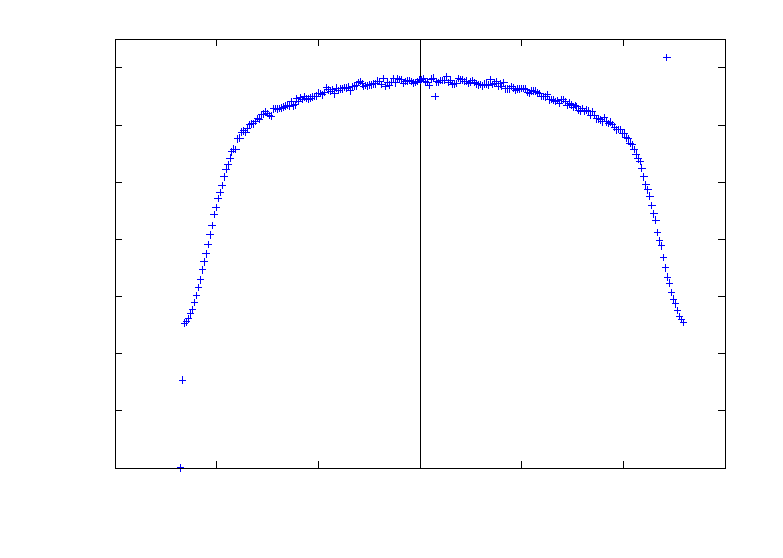
\includegraphics{plots/Sonnenspektrum}}%
    \gplfronttext
  \end{picture}%
\endgroup

        \caption[Beispielspektrum der Sonnenmessungen]{In dieser Abbildung ist beispielhaft ein aufgezeichnetes Sonnenspektrum gezeigt. Es handelt sich um die Messung, bei welcher sowohl Höhen- wie auch Azimutwinkelversatz gleich null sind. Dabei ist die Intensität über der Frequenz aufgetragen. Zudem wurde die Frequenz $\SI{1410}{\mega \hertz}$ markiert, bei welcher der zugehörige Intensitätswert ausgelesen wurde, da diese als Messfrequenz eingestellt wurde. Entsprechend wurden alle aufgezeichneten Spektren der Sonnenmessung analysiert.}
        \label{fig:Sonnenspektrum}
    \end{figure}

     

    Zur Einheit der Intensität sei angemerkt, dass diese stets in ,,arbitrary units`` bzw. in Kelvin (\SI{}{\kelvin}) angegeben wurden,
    da eine Kalibrierung des Teleskops für Absolutwerte vom \textsc{Onsala Space Observatory} nicht vorgenommen wurde.
    Allerdings genügt für die geforderten Belange eine Betrachtung der relativen Werte.\\

    \subsubsection{Raster-Scan der Sonne}
    Zunächst wurde ein Raster-Scan der Sonne vorgenommen, dabei wurden 25 Messungen zwischen $\SI{-10}{\degree}$ und $\SI{10}{\degree}$ Azimut- (azimuth) und Höhenwinkelversatz (altitude) in $\SI{5}{\degree}$-Schritten durchgeführt.
    Die entsprechenden jeweiligen Intensitätsmaxima wurden in Abbildung \ref{fig:Sonnenabbild} über den Relativwinkeln zur Sonne bei $\SI{0}{\degree}$ aufgetragen. 
    Die Interpolation zwischen den 25 Messwerten wurde dabei mittels \textSC{Gnuplot} durchgeführt. 
    \textsc{Gnuplot} verwendet hierbei den ,,Qnorm-Algorithmus``, welcher einen gewichteten Mittelwert der Messdaten an jedem Gitterpunkt berechnet. 
    Dabei wird jeder Messwert mit dem Inversen seines Abstands zum jeweiligen Gitterpunkt gewichtet. 
    Diese Gewichtung wird zudem mit der Ordnung der Norm des Abstands potenziert.
    Als zusätzliche Parameter können optional die Lage des erwarteten globalen Maximums und die erwartete Standardabweichung angegeben werden. 
    Die Lage wurde im Zentrum bei jeweils $\SI{0}{\degree}$ Azimutal- und Höhenwinkelversatz erkannt. 
    Auf die Angabe einer Standardabweichung wurde verzichtet.
    \begin{figure}[H]
        \centering
        % GNUPLOT: LaTeX picture with Postscript
\begingroup
  % Encoding inside the plot.  In the header of your document, this encoding
  % should to defined, e.g., by using
  % \usepackage[cp1252,<other encodings>]{inputenc}
  \inputencoding{cp1252}%
  \makeatletter
  \providecommand\color[2][]{%
    \GenericError{(gnuplot) \space\space\space\@spaces}{%
      Package color not loaded in conjunction with
      terminal option `colourtext'%
    }{See the gnuplot documentation for explanation.%
    }{Either use 'blacktext' in gnuplot or load the package
      color.sty in LaTeX.}%
    \renewcommand\color[2][]{}%
  }%
  \providecommand\includegraphics[2][]{%
    \GenericError{(gnuplot) \space\space\space\@spaces}{%
      Package graphicx or graphics not loaded%
    }{See the gnuplot documentation for explanation.%
    }{The gnuplot epslatex terminal needs graphicx.sty or graphics.sty.}%
    \renewcommand\includegraphics[2][]{}%
  }%
  \providecommand\rotatebox[2]{#2}%
  \@ifundefined{ifGPcolor}{%
    \newif\ifGPcolor
    \GPcolorfalse
  }{}%
  \@ifundefined{ifGPblacktext}{%
    \newif\ifGPblacktext
    \GPblacktexttrue
  }{}%
  % define a \g@addto@macro without @ in the name:
  \let\gplgaddtomacro\g@addto@macro
  % define empty templates for all commands taking text:
  \gdef\gplbacktext{}%
  \gdef\gplfronttext{}%
  \makeatother
  \ifGPblacktext
    % no textcolor at all
    \def\colorrgb#1{}%
    \def\colorgray#1{}%
  \else
    % gray or color?
    \ifGPcolor
      \def\colorrgb#1{\color[rgb]{#1}}%
      \def\colorgray#1{\color[gray]{#1}}%
      \expandafter\def\csname LTw\endcsname{\color{white}}%
      \expandafter\def\csname LTb\endcsname{\color{black}}%
      \expandafter\def\csname LTa\endcsname{\color{black}}%
      \expandafter\def\csname LT0\endcsname{\color[rgb]{1,0,0}}%
      \expandafter\def\csname LT1\endcsname{\color[rgb]{0,1,0}}%
      \expandafter\def\csname LT2\endcsname{\color[rgb]{0,0,1}}%
      \expandafter\def\csname LT3\endcsname{\color[rgb]{1,0,1}}%
      \expandafter\def\csname LT4\endcsname{\color[rgb]{0,1,1}}%
      \expandafter\def\csname LT5\endcsname{\color[rgb]{1,1,0}}%
      \expandafter\def\csname LT6\endcsname{\color[rgb]{0,0,0}}%
      \expandafter\def\csname LT7\endcsname{\color[rgb]{1,0.3,0}}%
      \expandafter\def\csname LT8\endcsname{\color[rgb]{0.5,0.5,0.5}}%
    \else
      % gray
      \def\colorrgb#1{\color{black}}%
      \def\colorgray#1{\color[gray]{#1}}%
      \expandafter\def\csname LTw\endcsname{\color{white}}%
      \expandafter\def\csname LTb\endcsname{\color{black}}%
      \expandafter\def\csname LTa\endcsname{\color{black}}%
      \expandafter\def\csname LT0\endcsname{\color{black}}%
      \expandafter\def\csname LT1\endcsname{\color{black}}%
      \expandafter\def\csname LT2\endcsname{\color{black}}%
      \expandafter\def\csname LT3\endcsname{\color{black}}%
      \expandafter\def\csname LT4\endcsname{\color{black}}%
      \expandafter\def\csname LT5\endcsname{\color{black}}%
      \expandafter\def\csname LT6\endcsname{\color{black}}%
      \expandafter\def\csname LT7\endcsname{\color{black}}%
      \expandafter\def\csname LT8\endcsname{\color{black}}%
    \fi
  \fi
    \setlength{\unitlength}{0.0500bp}%
    \ifx\gptboxheight\undefined%
      \newlength{\gptboxheight}%
      \newlength{\gptboxwidth}%
      \newsavebox{\gptboxtext}%
    \fi%
    \setlength{\fboxrule}{0.5pt}%
    \setlength{\fboxsep}{1pt}%
\begin{picture}(7200.00,5040.00)%
    \gplgaddtomacro\gplbacktext{%
    }%
    \gplgaddtomacro\gplfronttext{%
      \csname LTb\endcsname%%
      \put(963,1308){\makebox(0,0){\strut{}$-10$}}%
      \put(1773,1160){\makebox(0,0){\strut{}$-5$}}%
      \put(2583,1011){\makebox(0,0){\strut{}$0$}}%
      \put(3392,863){\makebox(0,0){\strut{}$5$}}%
      \put(4201,714){\makebox(0,0){\strut{}$10$}}%
      \put(2270,651){\rotatebox{-11}{\makebox(0,0){\strut{}azimuth offset in $\degree$}}}%
      \put(4427,746){\makebox(0,0)[l]{\strut{}$-10$}}%
      \put(4895,1004){\makebox(0,0)[l]{\strut{}$-5$}}%
      \put(5362,1261){\makebox(0,0)[l]{\strut{}$0$}}%
      \put(5830,1518){\makebox(0,0)[l]{\strut{}$5$}}%
      \put(6297,1775){\makebox(0,0)[l]{\strut{}$10$}}%
      \put(5903,960){\rotatebox{29}{\makebox(0,0){\strut{}altitude offset in $\degree$}}}%
      \put(920,1482){\makebox(0,0)[r]{\strut{}$300$}}%
      \put(920,1972){\makebox(0,0)[r]{\strut{}$400$}}%
      \put(920,2462){\makebox(0,0)[r]{\strut{}$500$}}%
      \put(920,2951){\makebox(0,0)[r]{\strut{}$600$}}%
      \put(920,3441){\makebox(0,0)[r]{\strut{}$700$}}%
      \put(122,2462){\rotatebox{90}{\makebox(0,0){\strut{}temperature in $\si{}{K}$}}}%
    }%
    \gplbacktext
    \put(0,0){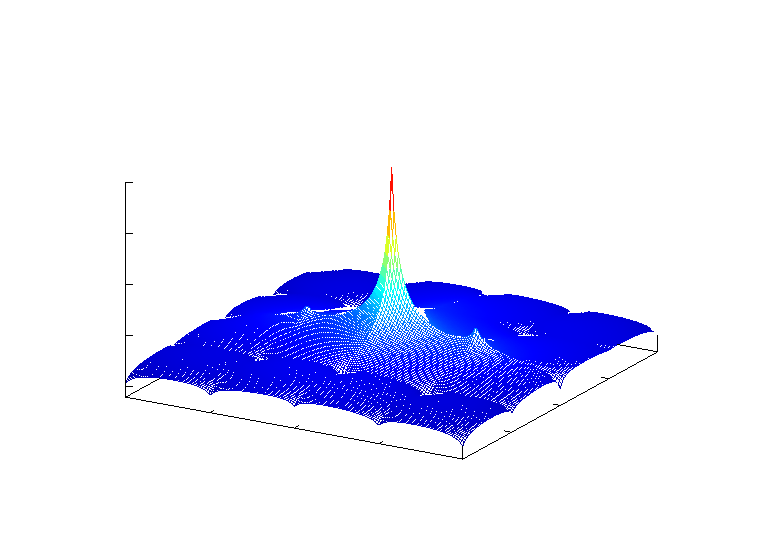
\includegraphics{plots/Sonnenabbild}}%
    \gplfronttext
  \end{picture}%
\endgroup

        \caption[Raster-Scan der Sonne]{Diese Abbildung zeigt den $5$$\times$$5$-Raster-Scan der Sonne. Dabei wird deutlich, dass in den dunkelblau gefärbten Bereichen von $>\vert \SI{5}{\degree}\vert$ Offset sowohl in Höhen- als auch in Azimutwinkel eine Grundintensität -- hier in \si{\kelvin} gemessen -- vorliegt. Die Sonne als Punktquelle aufzufassen, wird durch das ausgeprägte Intensitätsmaximum bei $\SI{0}{\degree}$ azimutalem und Höhenoffset legitimiert. Zudem fällt auf, dass bei $\SI{0}{\degree}$ Höhenoffset und $\vert\SI{5}{\degree}\vert$ azimutalem Offset erhöhte Intensitätswerte vorliegen, was bei entsprechendem Höhenwinkelversatz nicht zu erkennen ist. Dies lässt vermuten, dass es sich um ein $\sinc$-Profil handelt, die entsprechenden Maxima im Höhenwinkelversatz allerdings fehlen. Somit deutet dies ebenfalls auf eine Punktquelle hin.}
        \label{fig:Sonnenabbild}
    \end{figure}
    Die Farbskala veranschaulicht deutlich, dass in den äußeren Bereichen mit Relativwinkeln größer $\approx \vert \SI{5}{\degree}\vert$ eine Grundintensität von ca. $\SI{300}{\kelvin}$ vorliegt.
    Zum Zentrum hin nimmt die Intensität hingegen stark zu,
    wobei selbst die zentrumsnächsten Messungen bei $\vert\SI{5}{\degree}\vert$ lediglich in azimutaler Auslenkung leichte Erhöhungen aufweisen.
    Dies lässt die oben angedeutete Annahme zu, die Sonne hier als Punktquelle aufzufassen, da das in Abbildung \ref{fig:Sonnenabbild} zu sehende Beugungsbild einem dreidimensionalen $\sinc$-Profil gleicht. Wobei die Nebenmaxima in Richtung des Höhenwinkelversatzes fehlen.
    Dieses Beugungsbild erhält man, sofern sich das Radioteleskop wie eine Kreisblende und die Sonne wie eine Punktquelle verhalten. Auf Grundlage dieser Erkenntnis lassen sich im Folgenden daraus Standardabweichung, FWHM und das Auflösungsvermögen des Teleskops bestimmen.\\
    Auf die Darstellung von Unsicherheiten wurde zugunsten der Übersichtlichkeit verzichtet. Da nur qualitative Aussagen getroffen werden, sind Unsicherheitsbetrachtungen hinfällig.

    \subsubsection{Öffnungsfunktion des Radioteleskops}
    Zur Bestimmung der ,,antenna response function``,
    welche unter der Annahme, das Teleskop sei eine Lochblende, auch als Öffnungsfunktion verstanden werden kann,
    wurden zusätzlich zwei genauere Kreuzscans der Sonne aufgenommen.
    Hierfür wurde der Azimut- und Höhenoffset jeweils von $\SI{-16}{\degree}$ bis $\SI{16}{\degree}$ in $\SI{2}{\degree}$-Schritten variiert, wobei die jeweils andere Koordinate auf $\SI{0}{\degree}$ fixiert wurde.
    Die ausgelesenen Intensitätsmaxima wurden gegen den relativen Offset, bezogen auf die Sonne, aufgetragen.
    \begin{figure}[H]
        \centering
        % GNUPLOT: LaTeX picture with Postscript
\begingroup
  % Encoding inside the plot.  In the header of your document, this encoding
  % should to defined, e.g., by using
  % \usepackage[cp1252,<other encodings>]{inputenc}
  \inputencoding{cp1252}%
  \makeatletter
  \providecommand\color[2][]{%
    \GenericError{(gnuplot) \space\space\space\@spaces}{%
      Package color not loaded in conjunction with
      terminal option `colourtext'%
    }{See the gnuplot documentation for explanation.%
    }{Either use 'blacktext' in gnuplot or load the package
      color.sty in LaTeX.}%
    \renewcommand\color[2][]{}%
  }%
  \providecommand\includegraphics[2][]{%
    \GenericError{(gnuplot) \space\space\space\@spaces}{%
      Package graphicx or graphics not loaded%
    }{See the gnuplot documentation for explanation.%
    }{The gnuplot epslatex terminal needs graphicx.sty or graphics.sty.}%
    \renewcommand\includegraphics[2][]{}%
  }%
  \providecommand\rotatebox[2]{#2}%
  \@ifundefined{ifGPcolor}{%
    \newif\ifGPcolor
    \GPcolorfalse
  }{}%
  \@ifundefined{ifGPblacktext}{%
    \newif\ifGPblacktext
    \GPblacktexttrue
  }{}%
  % define a \g@addto@macro without @ in the name:
  \let\gplgaddtomacro\g@addto@macro
  % define empty templates for all commands taking text:
  \gdef\gplbacktext{}%
  \gdef\gplfronttext{}%
  \makeatother
  \ifGPblacktext
    % no textcolor at all
    \def\colorrgb#1{}%
    \def\colorgray#1{}%
  \else
    % gray or color?
    \ifGPcolor
      \def\colorrgb#1{\color[rgb]{#1}}%
      \def\colorgray#1{\color[gray]{#1}}%
      \expandafter\def\csname LTw\endcsname{\color{white}}%
      \expandafter\def\csname LTb\endcsname{\color{black}}%
      \expandafter\def\csname LTa\endcsname{\color{black}}%
      \expandafter\def\csname LT0\endcsname{\color[rgb]{1,0,0}}%
      \expandafter\def\csname LT1\endcsname{\color[rgb]{0,1,0}}%
      \expandafter\def\csname LT2\endcsname{\color[rgb]{0,0,1}}%
      \expandafter\def\csname LT3\endcsname{\color[rgb]{1,0,1}}%
      \expandafter\def\csname LT4\endcsname{\color[rgb]{0,1,1}}%
      \expandafter\def\csname LT5\endcsname{\color[rgb]{1,1,0}}%
      \expandafter\def\csname LT6\endcsname{\color[rgb]{0,0,0}}%
      \expandafter\def\csname LT7\endcsname{\color[rgb]{1,0.3,0}}%
      \expandafter\def\csname LT8\endcsname{\color[rgb]{0.5,0.5,0.5}}%
    \else
      % gray
      \def\colorrgb#1{\color{black}}%
      \def\colorgray#1{\color[gray]{#1}}%
      \expandafter\def\csname LTw\endcsname{\color{white}}%
      \expandafter\def\csname LTb\endcsname{\color{black}}%
      \expandafter\def\csname LTa\endcsname{\color{black}}%
      \expandafter\def\csname LT0\endcsname{\color{black}}%
      \expandafter\def\csname LT1\endcsname{\color{black}}%
      \expandafter\def\csname LT2\endcsname{\color{black}}%
      \expandafter\def\csname LT3\endcsname{\color{black}}%
      \expandafter\def\csname LT4\endcsname{\color{black}}%
      \expandafter\def\csname LT5\endcsname{\color{black}}%
      \expandafter\def\csname LT6\endcsname{\color{black}}%
      \expandafter\def\csname LT7\endcsname{\color{black}}%
      \expandafter\def\csname LT8\endcsname{\color{black}}%
    \fi
  \fi
    \setlength{\unitlength}{0.0500bp}%
    \ifx\gptboxheight\undefined%
      \newlength{\gptboxheight}%
      \newlength{\gptboxwidth}%
      \newsavebox{\gptboxtext}%
    \fi%
    \setlength{\fboxrule}{0.5pt}%
    \setlength{\fboxsep}{1pt}%
\begin{picture}(7200.00,5040.00)%
    \gplgaddtomacro\gplbacktext{%
      \csname LTb\endcsname%%
      \put(814,704){\makebox(0,0)[r]{\strut{}$300$}}%
      \put(814,1218){\makebox(0,0)[r]{\strut{}$350$}}%
      \put(814,1733){\makebox(0,0)[r]{\strut{}$400$}}%
      \put(814,2247){\makebox(0,0)[r]{\strut{}$450$}}%
      \put(814,2762){\makebox(0,0)[r]{\strut{}$500$}}%
      \put(814,3276){\makebox(0,0)[r]{\strut{}$550$}}%
      \put(814,3790){\makebox(0,0)[r]{\strut{}$600$}}%
      \put(814,4305){\makebox(0,0)[r]{\strut{}$650$}}%
      \put(814,4819){\makebox(0,0)[r]{\strut{}$700$}}%
      \put(1434,484){\makebox(0,0){\strut{}$-15$}}%
      \put(2248,484){\makebox(0,0){\strut{}$-10$}}%
      \put(3061,484){\makebox(0,0){\strut{}$-5$}}%
      \put(3875,484){\makebox(0,0){\strut{}$0$}}%
      \put(4688,484){\makebox(0,0){\strut{}$5$}}%
      \put(5501,484){\makebox(0,0){\strut{}$10$}}%
      \put(6315,484){\makebox(0,0){\strut{}$15$}}%
      \put(4851,2813){\makebox(0,0)[l]{\strut{}FWHM $ = \SI{7.80 \pm 0.13}{\degree}$}}%
      \put(4851,3173){\makebox(0,0)[l]{\strut{}$\sigma =  \SI{3.313 \pm 0.055}{\degree}$}}%
    }%
    \gplgaddtomacro\gplfronttext{%
      \csname LTb\endcsname%%
      \put(308,2761){\rotatebox{-270}{\makebox(0,0){\strut{}Intensit\"at in willk\"urlichen Einheiten}}}%
      \put(3874,154){\makebox(0,0){\strut{}Azimutwinkelversatz relativ zur Sonne in $\si{}{\degree}$}}%
      \csname LTb\endcsname%%
      \put(5816,4646){\makebox(0,0)[r]{\strut{}Messwerte}}%
      \csname LTb\endcsname%%
      \put(5816,4426){\makebox(0,0)[r]{\strut{}\textsc{Gauss}-Fit}}%
    }%
    \gplbacktext
    \put(0,0){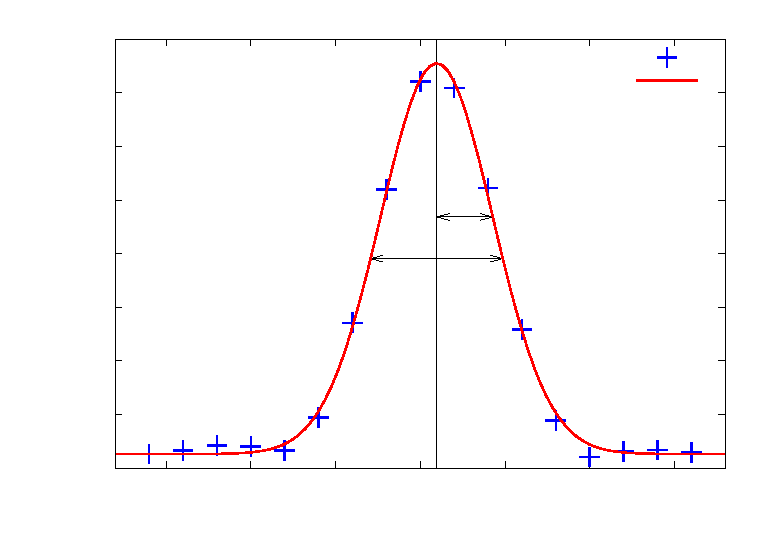
\includegraphics{plots/Sonnenkreuz_Az}}%
    \gplfronttext
  \end{picture}%
\endgroup

        \caption[Kreuz-Scan der Sonne, Azimutwinkelversatz]{Die Abbildung verdeutlicht den Verlauf der Datenpunkte gemäß einer $\sinc$-Funktion. Dies bestätigt die Annahme, das Radioteleskop als Lochblende aufzufassen, deren Öffnungsfunktion einer $\sinc$-Funktion entspricht. Zudem lassen sich mittels \textSC{Gauß}-Fit drei charakteristische Größen ermitteln: die Standardabweichung $\sigma$ als direktes Ergebnis des Fits mit \textsc{Gauß}scher Fehlerfunktion und die als spektrales Auflösungsvermögen zu verstehende FWHM, welche nach Formel \eqref{eq:FWHM} zu berechnen ist. Zudem kann ebenfalls direkt aus dem \textsc{Gauß}-Fit die Positioniergenauigkeit des Teleskops, welche auch als intrinsische Unsicherheit $d$ verstanden wird, abgelesen werden. Sie beziffert sich auf $d = \SI{0.968 \pm 0.047}{\degree}$.}
        \label{fig:Sonnenkreuz_Az}
    \end{figure}
    Die entsprechenden Darstellungen finden sich in Abbildung \ref{fig:Sonnenkreuz_Az} (azimutaler Offset) und Abbildung \ref{fig:Sonnenkreuz_Alt} (Höhenoffset).
    In beiden Abbildungen ist der charakteristische Verlauf der $\sinc$-Funktion zu erkennen.
    Dies bestätigt, dass sich das Teleskop wie eine Kreisblende verhält.
    Dabei bilden sich leichte lokale Maxima im Bereich von $\vert\SI{10}{\degree}\vert$ bis $\vert\SI{15}{\degree}\vert$ (Abb. \ref{fig:Sonnenkreuz_Az}) bzw. von $\vert\SI{6}{\degree}\vert$ bis $\vert\SI{10}{\degree}\vert$ (Abb. \ref{fig:Sonnenkreuz_Alt}) aus.
    \begin{figure}[H]
        \centering
        % GNUPLOT: LaTeX picture with Postscript
\begingroup
  % Encoding inside the plot.  In the header of your document, this encoding
  % should to defined, e.g., by using
  % \usepackage[cp1252,<other encodings>]{inputenc}
  \inputencoding{cp1252}%
  \makeatletter
  \providecommand\color[2][]{%
    \GenericError{(gnuplot) \space\space\space\@spaces}{%
      Package color not loaded in conjunction with
      terminal option `colourtext'%
    }{See the gnuplot documentation for explanation.%
    }{Either use 'blacktext' in gnuplot or load the package
      color.sty in LaTeX.}%
    \renewcommand\color[2][]{}%
  }%
  \providecommand\includegraphics[2][]{%
    \GenericError{(gnuplot) \space\space\space\@spaces}{%
      Package graphicx or graphics not loaded%
    }{See the gnuplot documentation for explanation.%
    }{The gnuplot epslatex terminal needs graphicx.sty or graphics.sty.}%
    \renewcommand\includegraphics[2][]{}%
  }%
  \providecommand\rotatebox[2]{#2}%
  \@ifundefined{ifGPcolor}{%
    \newif\ifGPcolor
    \GPcolorfalse
  }{}%
  \@ifundefined{ifGPblacktext}{%
    \newif\ifGPblacktext
    \GPblacktexttrue
  }{}%
  % define a \g@addto@macro without @ in the name:
  \let\gplgaddtomacro\g@addto@macro
  % define empty templates for all commands taking text:
  \gdef\gplbacktext{}%
  \gdef\gplfronttext{}%
  \makeatother
  \ifGPblacktext
    % no textcolor at all
    \def\colorrgb#1{}%
    \def\colorgray#1{}%
  \else
    % gray or color?
    \ifGPcolor
      \def\colorrgb#1{\color[rgb]{#1}}%
      \def\colorgray#1{\color[gray]{#1}}%
      \expandafter\def\csname LTw\endcsname{\color{white}}%
      \expandafter\def\csname LTb\endcsname{\color{black}}%
      \expandafter\def\csname LTa\endcsname{\color{black}}%
      \expandafter\def\csname LT0\endcsname{\color[rgb]{1,0,0}}%
      \expandafter\def\csname LT1\endcsname{\color[rgb]{0,1,0}}%
      \expandafter\def\csname LT2\endcsname{\color[rgb]{0,0,1}}%
      \expandafter\def\csname LT3\endcsname{\color[rgb]{1,0,1}}%
      \expandafter\def\csname LT4\endcsname{\color[rgb]{0,1,1}}%
      \expandafter\def\csname LT5\endcsname{\color[rgb]{1,1,0}}%
      \expandafter\def\csname LT6\endcsname{\color[rgb]{0,0,0}}%
      \expandafter\def\csname LT7\endcsname{\color[rgb]{1,0.3,0}}%
      \expandafter\def\csname LT8\endcsname{\color[rgb]{0.5,0.5,0.5}}%
    \else
      % gray
      \def\colorrgb#1{\color{black}}%
      \def\colorgray#1{\color[gray]{#1}}%
      \expandafter\def\csname LTw\endcsname{\color{white}}%
      \expandafter\def\csname LTb\endcsname{\color{black}}%
      \expandafter\def\csname LTa\endcsname{\color{black}}%
      \expandafter\def\csname LT0\endcsname{\color{black}}%
      \expandafter\def\csname LT1\endcsname{\color{black}}%
      \expandafter\def\csname LT2\endcsname{\color{black}}%
      \expandafter\def\csname LT3\endcsname{\color{black}}%
      \expandafter\def\csname LT4\endcsname{\color{black}}%
      \expandafter\def\csname LT5\endcsname{\color{black}}%
      \expandafter\def\csname LT6\endcsname{\color{black}}%
      \expandafter\def\csname LT7\endcsname{\color{black}}%
      \expandafter\def\csname LT8\endcsname{\color{black}}%
    \fi
  \fi
    \setlength{\unitlength}{0.0500bp}%
    \ifx\gptboxheight\undefined%
      \newlength{\gptboxheight}%
      \newlength{\gptboxwidth}%
      \newsavebox{\gptboxtext}%
    \fi%
    \setlength{\fboxrule}{0.5pt}%
    \setlength{\fboxsep}{1pt}%
\begin{picture}(7200.00,5040.00)%
    \gplgaddtomacro\gplbacktext{%
      \csname LTb\endcsname%%
      \put(814,704){\makebox(0,0)[r]{\strut{}$300$}}%
      \put(814,1218){\makebox(0,0)[r]{\strut{}$350$}}%
      \put(814,1733){\makebox(0,0)[r]{\strut{}$400$}}%
      \put(814,2247){\makebox(0,0)[r]{\strut{}$450$}}%
      \put(814,2762){\makebox(0,0)[r]{\strut{}$500$}}%
      \put(814,3276){\makebox(0,0)[r]{\strut{}$550$}}%
      \put(814,3790){\makebox(0,0)[r]{\strut{}$600$}}%
      \put(814,4305){\makebox(0,0)[r]{\strut{}$650$}}%
      \put(814,4819){\makebox(0,0)[r]{\strut{}$700$}}%
      \put(1434,484){\makebox(0,0){\strut{}$-15$}}%
      \put(2248,484){\makebox(0,0){\strut{}$-10$}}%
      \put(3061,484){\makebox(0,0){\strut{}$-5$}}%
      \put(3875,484){\makebox(0,0){\strut{}$0$}}%
      \put(4688,484){\makebox(0,0){\strut{}$5$}}%
      \put(5501,484){\makebox(0,0){\strut{}$10$}}%
      \put(6315,484){\makebox(0,0){\strut{}$15$}}%
      \put(4688,2864){\makebox(0,0)[l]{\strut{}FWHM $= \SI{5.63 \pm 0.12}{\degree}$}}%
      \put(4688,3276){\makebox(0,0)[l]{\strut{}$\sigma =  \SI{2.389 \pm 0.052}{\degree}$}}%
    }%
    \gplgaddtomacro\gplfronttext{%
      \csname LTb\endcsname%%
      \put(308,2761){\rotatebox{-270}{\makebox(0,0){\strut{}Kontinuums Intensität in willkürlichen Einheiten}}}%
      \put(3874,154){\makebox(0,0){\strut{}Höhenwinkelversatz relativ zur Sonne in $\si{}{\degree}$}}%
      \csname LTb\endcsname%%
      \put(5816,4646){\makebox(0,0)[r]{\strut{}Messwerte}}%
      \csname LTb\endcsname%%
      \put(5816,4426){\makebox(0,0)[r]{\strut{}\textsc{Gauss}-Fit}}%
    }%
    \gplbacktext
    \put(0,0){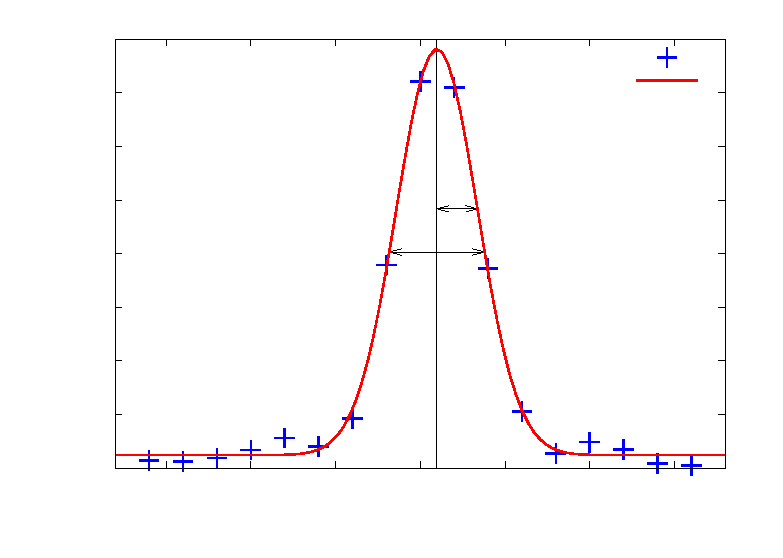
\includegraphics{plots/Sonnenkreuz_Alt}}%
    \gplfronttext
  \end{picture}%
\endgroup

        \caption[Kreuz-Scan der Sonne, Höhenwinkelversatz]{Analog zu Abbildung \ref{fig:Sonnenkreuz_Az} ist hier die Messung bei variiertem Höhenwinkelversatz dargestellt. Die Standardabweichung ($\sigma$), FWHM sowie die intrinsische Unsicherheit ($d = \SI{0.984 \pm 0.048}{\degree}$) berechnen sich entsprechend.}
        \label{fig:Sonnenkreuz_Alt}
    \end{figure}
    An die Datenpunkte wurde jeweils eine \textsc{Gauß}-Funktion angefittet, welcher dann weitere Berechnungen folgten.
    % Welcher Parameter????
    Der Erwartungswert $d$ lässt einen Rückschluss auf Abweichungen in der Positioniergenauigkeit des Teleskops zu und kann hier somit als intrinsische Unsicherheit aufgefasst werden.
    Diese umfasst beispielsweise äußere Einflüsse, wie ein Zittern des Teleskops aufgrund von Wind oder auch der Umstand, dass das Teleskop in Schritten von $\SI{0.125}{\degree}$ trackt \cite{Usermanual}. Auch die Erdrotation ruft eine Winkeländerung mit $\approx \SI{0.25}{\degree}$ pro Minute hervor.
    Diese ,,tracking accuracy`` beträgt nach \cite{Usermanual} $\SI{0.5}{\degree}$. 
    Aus den beiden Messreihen ergab sich nach Bilden des gewichteten Mittelwerts und der zugehörigen Unsicherheit auf Grundlage der aus den mittels \textsc{Gnuplot} gewonnenen Größen und zugehörigen Unsicherheiten ein Wert von $d = \SI{0.976 \pm 0.034}{\degree}$.
    Somit liegt der hier gefundene Wert der Positioniergenauigkeit, auch im Rahmen der berechneten Unsicherheiten, höher als der aus der Literatur erwartete Wert. 
    Dennoch lässt die korrekte Größenordnung auf eine fehlerfreie Vorgehensweise schließen.
    Es lässt sich lediglich für die weiteren Beobachtungen festhalten, dass bei den hier gegebenen Bedingungen vermutlich etwas größere Unsicherheiten vorlagen aufgrund von beispielsweise kurzen Messzeiten oder starkem Wind. 
    Zudem ist das Teleskop bereits seit mehreren Jahren der örtlichen Witterung ausgesetzt.
    Dies könnte trotz Wartungsarbeiten zu leichten Schäden der Mechanik oder einer leicht fehlerhaften Justierung des Teleskops geführt haben.
    
    Möglichkeiten, um noch präzisere Ergebnisse zu erhalten, wären in Bezug auf die Messung selbst die Anzahl und Integrationszeit der Messungen zu erhöhen, um mehr Daten zu generieren. Um eine fehlerhafte Justierung oder Schäden an der Mechanik zu beheben, könnten regelmäßigere Wartungsarbeiten Potenzial bergen. Wohingegen auf das Wetter kein Einfluss genommen werden kann.\\ 


    Nun soll das spektrale Auflösungsvermögen genauer berechnet und mit der in der Literatur angegebenen ,,tracking accuracy`` verglichen werden.
    Aus der beim \textsc{Gauß}schen Fit gewonnenen Standardabweichung $\sigma$ konnte zunächst die Halbwertsbreite FWHM nach \cite{FWHM}
    \begin{align}
        \text{FWHM} = \sigma \cdot 2\sqrt{2\ln(2)} \label{eq:FWHM}
    \end{align}
    berechnet werden.
    Diese kann direkt als spektrales Auflösungsvermögen verstanden werden.
    Die entsprechenden Werte sind den beiden Abbildungen \ref{fig:Sonnenkreuz_Az} und \ref{fig:Sonnenkreuz_Alt} zu entnehmen. Hierbei wurden ebenfalls der gewichtete Mittelwert gebildet und die zugehörige Unsicherheit bestimmt.
    Somit ergab sich ein Wert von $\text{FWHM} = \SI{6.6 \pm 1.1}{\degree}$, welcher ebenfalls auf Grundlage der berechneten Unsicherheit in guter Übereinstimmung mit dem Literaturwert von $\approx \SI{6}{\degree}$ \cite{Usermanual} liegt. 
    Dieser Wert übersteigt die vorab bestimmte Positioniergenauigkeit deutlich und unterstreicht somit, dass diese im Vergleich zum spektralen Auflösungsvermögen vernachlässigbar ist.

    Anhand der gewonnenen Werte des Auflösungsvermögens (FWHM) aus den beiden Messreihen konnte nach dem \textsc{Rayleigh}-Kriterium mittels folgender Gleichung zudem auf den Durchmesser $D$ des Teleskops geschlossen werden \cite{Karttunen2013}:
    \begin{align}
        \Theta &= 1.22 \, \frac{\lambda}{D} \approx \ang{;;2.52} \times \frac{\lambda}{\SI{100}{\nano \metre}} \frac{\SI{1}{\centi \metre}}{D} = \SI{70}{\degree} \, \frac{\lambda}{D}\\
        \Leftrightarrow \quad D &= \SI{70}{\degree} \, \frac{\lambda}{\theta}.
    \end{align}
    Hierbei bezeichnet $\Theta$ das spektrale Auflösungsvermögen, welches durch FWHM gegeben ist. Für die Wellenlänge $\lambda$ wurde über $c = \lambda \cdot f$ die bekannte Frequenz $f$ eingesetzt und $D$ bezeichnet den Teleskopdurchmesser.
    Der Vorfaktor geht dabei aus der Bestimmung der Nullstellen der dem \textsc{Rayleigh}-Kriterium zugrunde liegenden \textsc{Bessel}funktionen hervor und wurde in das Gradmaß umgerechnet.

    Dabei ergaben sich die Werte $D_{\text{az}} = \SI{1.895 \pm 0.032}{\metre}$ und $D_{\text{alt}} = \SI{2.625 \pm 0.056}{\metre}$ für die azimutale (az) und Höhenkomponente (alt).
    Die jeweilig zugehörigen kombinierten Standardunsicherheiten wurden dabei nach 
    \begin{align}
        u_{\text{c}}(D) = \frac{\mathrm{d} D(\theta)}{\mathrm{d} \theta} \cdot u(\theta)
    \end{align}
    berechnet.
    Hierbei fällt im Hinblick auf den Literaturwert $D = \SI{2.3}{\metre}$ (\cite{Usermanual}) auf, dass beide Werte auf Grundlage ihrer Unsicherheiten nicht mit diesem vereinbar sind. 
    Zudem deuten die erhaltenen Werte auf ein nicht kreisförmiges oder unsymmetrisches Teleskop hin. 
    Dafür bestehen mehrere Erklärungsansätze. 
    Zum einen könnte ein durch den Wind verursachtes Wackeln des Teleskops die Messungen beeinflusst haben, dies würde allerdings eher den größeren Wert von $D_{\text{alt}}$ erklären. 
    Dahingehend könnten die Messungen beispielsweise durch noch kleinschrittigere Variationen in Azimut- und Höhenwinkelversatz verbessert werden.
    Wiederum könnten auch mechanische Schäden Einfluss auf die Messungen genommen haben. 
    Zum anderen ist in Betracht zu ziehen, dass das Teleskop nach mehreren Jahren der Nutzung einige kleine Defekte aufweisen könnte. 
    So könnten Elemente des Parabolspiegels womöglich nicht mehr zu den Messungen beitragen und damit die effektive Messleistung verringern. 
    Sollten sich diese Defekte auf einen bestimmten Bereich des Teleskops konzentrieren, könnte dies den geringen Wert der azimutalen Komponente erklären.
    Auch könnte die Positioniergenauigkeit des Teleskops in eine Richtung größer sein als in die andere.
    Um solchen Defekten entgegenzuwirken, wären Wartungen am Teleskop oder eine verbesserte Justierung unter Berücksichtigung der Defekte hilfreich.
    Zudem könnten Testmessungen durchgeführt werden, um zu ergründen, worauf der Unterschied in den beiden Komponenten zurückzuführen ist.

    Zuletzt sei erwähnt, dass die zugehörigen Unsicherheiten sowohl von $D_{\text{az}}$ wie auch von $D_{\text{alt}}$ recht gering ausfallen. Dies liegt im kleinen Wert der Unsicherheit der FHWM begründet, welcher \textSC{Gnuplot} entnommen wurde.

    Anschließend wurde der gewichtete Mittelwert der beiden berechneten Werte des Teleskopdurchmessers gebildet.
    Da die Grundlage der durch den \textsc{Gauß}-Fit gewonnenen Größen eine nicht geringe Anzahl an einzelnen Messwerten darstellt, wurde statt der recht gering ausfallenden kombinierten Unsicherheit die Standardabweichung der erhaltenen Teleskopdurchmesser berechnet und als sinnvoll erachtet.
    Somit konnte der Durchmesser des Radioteleskops ,,Brage`` aus den erhaltenen Daten bestimmt werden und beziffert sich auf $D = \SI{2.23 \pm 0.37}{\metre}$. Dieser Wert liegt in guter Übereinstimmung zu dem in der Projekt-Dokumentation \cite{Usermanual} genannten Wert von $D = \SI{2.3}{\metre}$. \\    
    
    Somit kann konstatiert werden, dass die Messungen während des Versuchstags mit hinreichend großer Präzision durchgeführt und einige charakteristische Größen des Teleskops bestätigt werden konnten.